\section{Photometric Redshifts}\label{mlg_sec:pz_summary}

For each observing strategy from {\tt OpSim} and {\tt ALTSched}, we evaluated the evolution in photometric depth of extragalactic fields (i.e., constraints on Galactic dust extinction and coordinates) that were associated with the wide-fast-deep (WFD) main survey. Only observing strategies that result in photometric depths that differ significantly from the baseline cadence will result in significantly different photometric redshifts using the color-matched nearest neighbors (CMNN) code presented by \cite{2018AJ....155....1G}. The six observing strategies for which we simulated photo-$z$ results are: the {\tt OpSim} baseline ({\tt kraken\_2026}), the {\tt OpSim} extended PanSTARRs-like WFD area of $24,700$ square degrees ({\tt pontus\_2002}), the {\tt OpSim}  ``many visits" strategy with 20/40 second exposures in $grizy$/$u$ filters ({\tt pontus\_2489}), the {\tt OpSim} rolling cadence with two declination bands prioritized in alternating years and in which the deprioritized band still receives $25\%$ of the baseline visits, the {\tt ALTSched} baseline cadence, and the {\tt ALTSched} rolling cadence which also observes alternating declination bands but allots no visits to the deprioritized area. We use the distribution of predicted $5{\sigma}$ liming magnitudes in sky HEALpix, each about the size of a single LSST pointing, to simulate observed apparent magnitudes for a test set of galaxies (the training set is simulated with the baseline's average $5{\sigma}$ liming magnitudes in all experiments). We then use the CMNN photo-$z$ estimator to simulate the photometric redshift results from each of the six considered observing strategies. We do this for LSST years 1, 3, 6, and 10.

To evaluate our results, we first reject catastrophic outliers with $|z_{\rm true}-z_{\rm phot}|>1.5$, and then 
calculate the robust standard deviation in the photo-$z$ error, $\Delta z _{1+z} = (z_{\rm true}-z_{\rm phot})/(1+z_{\rm 
phot})$, as the FWHM of the interquartile range (IQR) divided by $1.349$. (The fraction of outliers is captured by a 
different statistic not included in this short summary). We calculate this statistic for a low-$z_{\rm phot}$ bin 
(0.8-1.2) and a high-$z_{\rm phot}$ bin (1.8-2.2), for each of our considered observing strategies, for LSST years 1, 3, 
6, and 10. The resulting evolution in robust standard deviation for LSST photo-$z$ for each strategy is plotted as a 
function of survey year in Figure \ref{fig:evol}.

We can see immediately that the {\tt ALTSched} rolling cadence (black) offers significantly improved results in the half of the sky it does survey in year 1, but that by year 10 its results have converged with the other strategies. We can also see that the extended WFD area survey causes a significant degradation in the photo-$z$ results at all times (green line), and that the 20/40 second visits option outperforms the other strategies in the high-$z$ bin (orange line), {\it including the baseline cadence}. This can be attributed mainly to the deeper $u$-band images produced by this strategy, which are beneficial to photo-$z$ estimates.

\begin{figure}[h]
\begin{center}
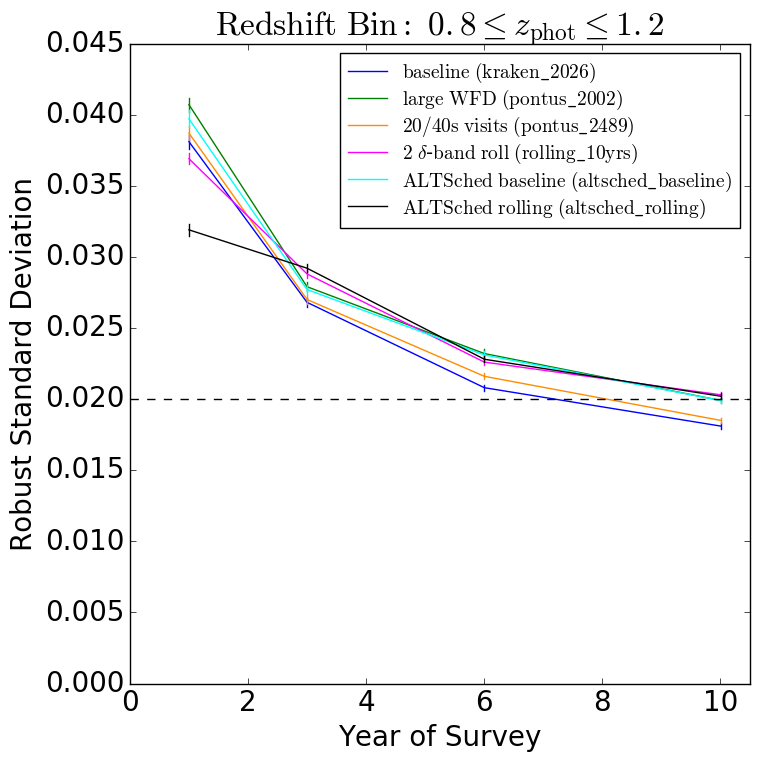
\includegraphics[width=7cm,trim={0cm 0cm 0cm 0cm},clip]{figures/zbin1_IQRs.png}
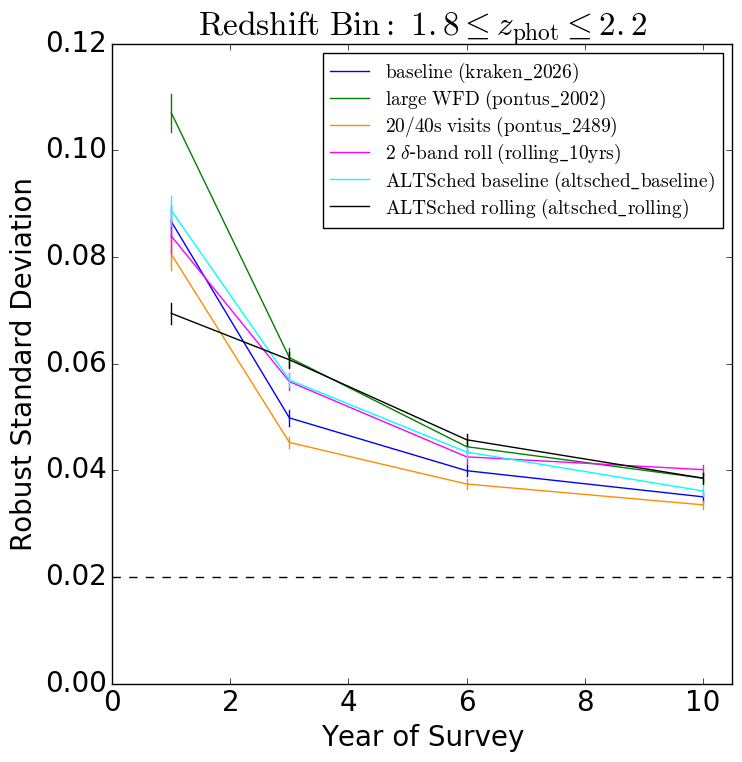
\includegraphics[width=7cm,trim={0cm 0cm 0cm 0cm},clip]{figures/zbin2_IQRs.png}
\caption{Statistical measures of the photo-$z$ robust standard deviation (after rejecting catastrophic outliers, calculated from the width of the intraquartile range) as a function of the LSST survey year, for two bins of photometric redshift: $0.8 \leq z_{\rm phot} \leq 1.2$ (left) and  $1.8 \leq z_{\rm phot} \leq 2.2$ (right). Results are presented for the {\tt OpSim} baseline ({\tt kraken\_2026}; blue), large WFD area with declinations including  $-78<\delta<+18$ degrees ({\tt pontus\_2002}; green), the ``many visits" strategy with 40/20 second exposures in $u$/$grizy$ filters ({\tt pontus\_2489}; orange), and a rolling cadence with two declination bands ({\tt rolling\_10yrs}; magenta), as well as for the {\tt ALTSched} results for a baseline (cyan) and rolling (black) cadence. Horizontal dashed line represents the LSST Science Requirement Document's target for a photo-$z$ bin of $0.3 \leq z_{\rm phot} \leq 3.0$. \label{fig:evol}}
\end{center}
\end{figure}
